\documentclass[11pt,a4paper]{article}

% ── Core packages ────────────────────────────────────────────────────────────
\usepackage[margin=1in]{geometry}
\usepackage{graphicx}
\usepackage[table]{xcolor}
\usepackage{colortbl}
\usepackage{booktabs}
\usepackage{tabularx}
\usepackage{float}
\usepackage{enumitem}
\usepackage{longtable}
\usepackage{amsmath, amssymb}
\usepackage{array}
\usepackage{titlesec}
\usepackage{fancyhdr}
\usepackage{microtype}
\usepackage[colorlinks=true, linkcolor=blue, urlcolor=blue, citecolor=blue]{hyperref}
\usepackage[most]{tcolorbox}

% ── List compaction ──────────────────────────────────────────────────────────
\setlist[itemize]{nosep, leftmargin=*, topsep=2pt, partopsep=0pt}
\setlist[enumerate]{nosep, leftmargin=*, topsep=2pt, partopsep=0pt}

% ── Widow / orphan penalties ─────────────────────────────────────────────────
\widowpenalty=10000
\clubpenalty=10000

% ── Colours ──────────────────────────────────────────────────────────────────
\definecolor{primary}{RGB}{31, 73, 125}
\definecolor{accentcol}{RGB}{0, 112, 192}
\definecolor{lightbg}{RGB}{235, 241, 251}
\definecolor{warnbg}{RGB}{255, 243, 205}
\definecolor{warnframe}{RGB}{180, 120, 0}
\definecolor{successbg}{RGB}{209, 231, 221}
\definecolor{successframe}{RGB}{25, 135, 84}

% ── Section headings ────────────────────────────────────────────────────────
\titleformat{\section}
  {\large\bfseries\color{primary}}{}{0em}{}[\titlerule]
\titleformat{\subsection}
  {\normalsize\bfseries\color{accentcol}}{}{0em}{}
\titlespacing*{\section}{0pt}{14pt}{6pt}
\titlespacing*{\subsection}{0pt}{10pt}{4pt}

% ── Headers / footers ────────────────────────────────────────────────────────
\pagestyle{fancy}
\fancyhf{}
\lhead{\small\textcolor{gray}{Neural MCPF Allocation --- Project Status Report}}
\rhead{\small\textcolor{gray}{June 2026}}
\cfoot{\small\thepage}
\renewcommand{\headrulewidth}{0.4pt}

% ── Coloured callout boxes (tcolorbox — robust across TeX Live versions) ──────
\newtcolorbox{execbox}[1]{breakable, colback=lightbg, colframe=primary, boxrule=1pt,
  arc=1pt, left=8pt, right=8pt, top=6pt, bottom=6pt,
  before upper={\textbf{\color{primary}#1}\par\smallskip}}

\newtcolorbox{findingbox}[1]{breakable, colback=successbg, colframe=successframe, boxrule=1pt,
  arc=1pt, left=8pt, right=8pt, top=6pt, bottom=6pt,
  before upper={\textbf{\color{successframe}#1}\par\smallskip}}

\newtcolorbox{warnbox}[1]{breakable, colback=warnbg, colframe=warnframe, boxrule=1pt,
  arc=1pt, left=8pt, right=8pt, top=6pt, bottom=6pt,
  before upper={\textbf{\color{warnframe}#1}\par\smallskip}}

% ─────────────────────────────────────────────────────────────────────────────
\begin{document}

% ── Title block ──────────────────────────────────────────────────────────────
\begin{center}
{\LARGE\bfseries\color{primary} Neural MCPF Allocation}\\[4pt]
{\large Project Status Report --- Implementation \& Benchmarking Phase}\\[6pt]
{\normalsize Course: Multi-Agent Systems \quad\textbar\quad June 2026}
\end{center}
\vspace{6pt}
{\color{primary}\hrule height 1.2pt}
\vspace{10pt}

% ═════════════════════════════════════════════════════════════════════════════
\section{Executive Summary}
% ═════════════════════════════════════════════════════════════════════════════

\begin{execbox}{Project Status}
The Neural MCPF Allocation project has completed eleven successive experiments, demonstrating
that a compact transformer network can replicate the goal-allocation decisions of an exact
combinatorial solver (RobustMCPF / LKH-TSP) at \textbf{2--4$\times$ single-instance speedup}
and \textbf{1--6\% execution-cost overhead} across 28 problem configurations
(N$\in$\{2,3,4,5\} agents, M$\in$\{2,\ldots,8\} goals, 8$\times$8 grids). The most recent phase
scales the model to 1.2M parameters and trains it on a diverse grid distribution, achieving
a mean execution-cost ratio of \textbf{1.020} with 0\% infeasible allocations across 5,600 test
instances.
\end{execbox}

\begin{execbox}{Phase Two --- Real Benchmark Maps (Exps 12--15)}
The project then moved onto the four 32$\times$32 RobustMCPF benchmark maps (open, scattered,
maze, rooms) at paper scale (N$\in$\{5,10,15\}, M$\in$\{10,20,30\}). Key results: map-trained
models reach \textbf{1.048} mean execution-cost ratio; the old small-scale model
\emph{generalizes across map geometry but not across N/M scale}; training on cheap random grids
\emph{matches} fixed-map training everywhere \emph{except the structured maze}; and at extreme
scale (N$\le$50, M$\le$100) the larger model wins with \textbf{5.9--9.4$\times$} speedup --- the
regime where replacing the solver pays off most.
\end{execbox}

% ═════════════════════════════════════════════════════════════════════════════
\section{Key Achievements}
% ═════════════════════════════════════════════════════════════════════════════

\textbf{Architecture selection (Exp 1).} A systematic comparison of three architectures on the
base task (N=2, M=2, 5$\times$5 grid) established the Transformer as the dominant model. It
outperforms MLP and DeepSets on every metric, and its advantage over MLP grows from 1.7 pt at
N=2 to 6.7 pt at N=5 --- indicating that the attention mechanism better captures the combinatorial
structure of larger problems.

\textbf{Critical feature discovery (Exp 5).} Adding goal-to-goal BFS distances
$G\in\mathbb{R}^{M\times M}$ to the input lifted full-assignment accuracy by \textbf{14--18
percentage points} across all agent counts. This single input change outweighed every
architecture, capacity, and data-scale improvement combined by a factor of $>10\times$.

\textbf{Universal mixed-size model (Exp 7).} A single 151k-parameter transformer trained jointly
on 15 problem configurations achieved zero-shot transfer to unseen N=5 problems, matching or
exceeding per-size specialists trained specifically on those sizes.

\textbf{Full-pipeline integration (Exps 8--10).} The NN allocation module was integrated into
the complete MAPF pipeline (NN forward pass $\to$ tour ordering $\to$ CBS collision planning),
enabling end-to-end execution-cost benchmarks against the full solver across all 28 configurations
at 200 instances each. Zero instances were ultimately infeasible after the probability-ranked
fallback chain.

\textbf{Large-model scale-up (Exp 11).} A 1.2M-parameter model trained on diverse grids (sizes
8--12, wall density 0.1--0.5, all 28 N$\times$M pairs) reduced the mean execution-cost ratio
to \textbf{1.020} on its training distribution, improved hard high-$M$ cells by 2--3 points,
and produced zero infeasible allocations.

% ═════════════════════════════════════════════════════════════════════════════
\section{Technical Progress \& Methodology}
% ═════════════════════════════════════════════════════════════════════════════

\subsection{Problem Formulation}

The project treats goal allocation as a multi-agent Travelling Salesman Problem (mTSP): given
$N$ agents on a grid with $M$ goals, assign every goal to exactly one agent so as to minimize
the total tour cost. Unlike balanced assignment, agents are unconstrained in the number of goals
they receive --- the solver may assign both goals to one agent when doing so is cheaper than
splitting them. Ground-truth labels are produced by RobustMCPF running LKH-TSP in BasicMAPF
mode; the neural network imitates these labels and replaces the solver's allocation step at
inference time.

The network input $D \in \mathbb{R}^{N \times M}$ is the BFS shortest-path distance matrix
from each agent to each goal, normalized to $[0,1]$. A secondary input $G \in \mathbb{R}^{M \times M}$
captures goal-to-goal distances and is injected via a learned projection. The output
$P \in \mathbb{R}^{N \times M}$ is a column-wise softmax: for each goal $j$,
$\sum_i P_{ij} = 1$, giving the probability that agent $i$ visits goal $j$.

\subsection{Loss Function}

Training minimizes a composite loss:
\[
\mathcal{L} = \mathcal{L}_{CE} + \lambda \cdot \mathcal{L}_{MinSum}
\]
\noindent where $\mathcal{L}_{CE}$ is per-goal cross-entropy over agents (solver imitation),
$\mathcal{L}_{MinSum} = \frac{1}{M}\sum_{i,j} P_{ij} D_{ij}$ penalizes distant assignments,
and $\lambda = 0.1$. The cross-entropy term dominates in practice; the MinSum regularizer
prevents degenerate uniform predictions early in training.

\subsection{Architecture Evolution}

Three architectures were evaluated. \textbf{GoalAllocMLP} flattens the input matrix and applies
two hidden layers. \textbf{GoalAllocDeepSets} applies a shared per-goal MLP.
\textbf{GoalAllocTransformer} applies alternating row--column attention on $D$ with per-size
positional embeddings. A fourth variant, \textbf{GoalAllocTransformerUniversal}, removes
positional embeddings entirely and injects $G$ via scalar embedding plus sum-pooling, making
the model size-agnostic and enabling mixed-size training over heterogeneous $(N,M)$ batches
without padding.

\subsection{Data Pipeline}

Datasets are generated by placing agents and goals uniformly on random obstacle grids and calling
the solver to produce labels. A BFS reachability filter discards instances where any goal is
unreachable. In Exp 11, a CBS node budget (50k expansions per call) additionally rejects
instances where constraint-dense mazes would prevent solver termination --- a condition encountered
in 12 of 28 generation tasks at 50\% wall density. The pipeline supports configurable grid
dimensions, wall densities, and $(N,M)$ pairs, with parallel worker processes to offset the
30--65 ms per-instance solver overhead.

\subsection{Training Configuration}

All experiments use Adam with ReduceLROnPlateau and 100 epochs unless noted. Exp 11 uses
lr$=5\times10^{-4}$, gradient clipping at 1.0, and 150 epochs on 840k training samples
(30k per configuration across all 28 pairs). A \texttt{MixedSizeBatchSampler} ensures each
batch is shape-homogeneous. Hardware: NVIDIA RTX 3090; training time $\sim$25 min/seed for the
small model, $\sim$3 h/seed for the large model.

% ═════════════════════════════════════════════════════════════════════════════
\section{Blockers \& Challenges}
% ═════════════════════════════════════════════════════════════════════════════

\textbf{Seed leakage (resolved).} Before 2026-06-11, the dataset builder seeded every split
with the same base seed, causing validation and test instances to replay the training set's RNG
stream. The original PoC numbers (per-goal 0.855, full-assignment 0.720) were measured on
contaminated test sets and are void. The fix introduces per-split seeding; a regression test in
\texttt{tests/test\_build\_dataset.py} guards against recurrence.

\textbf{CBS non-termination on dense mazes (resolved).} At wall densities up to 50\%, CBS can
enter an infinite constraint-escalation loop on instances where no collision-free plan exists.
This halted 12 of 28 data-generation tasks in Exp 11 and one evaluation instance in Exp 10.
A 50k-node expansion budget now terminates CBS early; budget-exceeded instances are rejected
during generation or resolved via the probability-ranked fallback chain at inference.

\textbf{LKH binary portability.} The LKH TSP binary is not committed to the repository
(platform-specific). Cluster jobs invoke \texttt{scripts/setup\_robustmcpf.sh} on first run,
adding a one-time build cost on any new cluster node.

\begin{warnbox}{Metric Caveat}
The offline cost ratio in Exps 1--7 is a first-hop proxy ($\sum P_{ij} D_{ij}$), not the
true mTSP tour cost. Values below 1.0 in that metric reflect the metric mismatch, not
super-solver performance. Full-pipeline experiments (Exps 8--11) use real CBS execution cost
and are directly interpretable: ratio 1.0 means the NN matches the exact solver.
\end{warnbox}

\textbf{Brute-force tour ordering.} The NN pipeline enumerates all $k!$ visit orders for each
agent's assigned goals. At $k=7$ or $k=8$ this dominates pipeline latency (38 ms for n2m8,
41 ms for n5m5), masking the NN's allocation speed advantage. A learned ordering step would
eliminate this bottleneck.

% ═════════════════════════════════════════════════════════════════════════════
\section{Data \& Metrics}
% ═════════════════════════════════════════════════════════════════════════════

\subsection{Metric Definitions}

The experiments report two families of metrics. \emph{Allocation-quality} metrics (per-goal
and full-assignment accuracy, computed in \texttt{evaluation/evaluate.py}) compare the NN's
predicted assignment against the solver's ground-truth assignment, with no path planning
(Exps 1--7). \emph{Execution-cost} metrics (cost ratio, exact match, diff, speedup,
infeasible/fallback, computed in \texttt{evaluation/full\_pipeline\_eval.py}) run each pipeline
end-to-end through CBS path planning and compare the resulting plans (Exps 8--11).

\paragraph{Notation.} For one instance the network outputs $P\in[0,1]^{N\times M}$ --- each
column a distribution over the $N$ agents, $\sum_i P_{ij}=1$ --- and the solver gives ground
truth $Y\in\{0,1\}^{N\times M}$, each column one-hot. Write the predicted and true agent for
goal $j$ as $\hat a_j=\arg\max_i P_{ij}$ and $a^\star_j=\arg\max_i Y_{ij}$, and the decoded hard
allocation as $\hat Y_{ij}=\mathbb{1}[i=\hat a_j]$. $D\in\mathbb{R}^{N\times M}$ is the
agent$\to$goal BFS distance matrix, and $\langle\,\cdot\,\rangle$ denotes the arithmetic mean
over the $S$ test instances of a configuration. $\mathbb{1}[\cdot]$ is the 0/1 indicator.

\medskip
\noindent\textbf{Allocation-quality metrics} (Exps 1--7) compare the predicted and ground-truth
allocations directly, with no path planning. \emph{Per-goal accuracy} is the fraction of
individual goals routed to the solver's chosen agent: per instance it is
$\frac{1}{M}\sum_{j=1}^{M}\mathbb{1}[\hat a_j=a^\star_j]$, and the reported figure is the mean of
this over all test instances, $\langle\cdot\rangle$. It is lenient --- one wrong goal in an
$M$-goal instance still scores $(M{-}1)/M$ --- and because $M$ is fixed within a configuration it
equals the overall share of correctly assigned goals. \emph{Full-assignment accuracy} is the
strict counterpart: the per-instance score is the all-or-nothing indicator
$\mathbb{1}[\hat Y = Y]$, equal to $1$ only when every one of the $M$ decoded columns matches the
solver, so its mean over instances empirically tracks (per-goal accuracy)$^{M}$. \emph{Cost ratio
(proxy)} compares only the first-hop BFS cost of the two allocations: per instance it is the ratio
$\big(\sum_{ij} D_{ij}\hat Y_{ij}\big)\big/\big(\sum_{ij} D_{ij} Y_{ij}\big)$ --- NN cost over
solver cost, set to $1$ when the solver cost underflows below $10^{-9}$ --- and these per-instance
ratios are then averaged. Because it ignores tour chaining and collisions, values below $1.0$
reflect the metric mismatch, not the NN beating the solver.

\medskip
\noindent\textbf{Execution-cost metrics} (Exps 8--11) instead run both pipelines end-to-end and
compare the resulting plans, where the cost $c$ of a plan is the total collision-free path length
in integer grid steps that CBS returns after resolving every conflict (the solver's
\texttt{Solution[5]}). \emph{Cost ratio (execution)} is the per-instance ratio
$c_{\mathrm{nn}}/c_{\mathrm{sol}}$ averaged over instances: $1.0$ means the NN matches the optimal
solver and $1.05$ is $5\%$ costlier. \emph{Exact match} is the fraction of instances whose two
integer costs are exactly equal, $\langle\mathbb{1}[c_{\mathrm{nn}}=c_{\mathrm{sol}}]\rangle$; it
runs higher than full-assignment accuracy because many distinct allocations are cost-equivalent
ties (for example, two agents equidistant from a goal). \emph{Diff (steps)} is the mean signed gap
$\langle c_{\mathrm{nn}}-c_{\mathrm{sol}}\rangle$ in grid steps, zero on an exact match, and the
same per-instance differences also produce the std and max quoted in the logs. \emph{Speedup} is
the ratio of \emph{mean} single-instance wall-times,
$\langle t_{\mathrm{sol}}\rangle/\langle t_{\mathrm{nn}}\rangle$ --- a ratio of means, not the mean
of per-instance ratios --- where $t_{\mathrm{nn}}$ covers the forward pass, goal-visit ordering and
CBS, and $t_{\mathrm{sol}}$ covers LKH-TSP and CBS on the same CPU node. Finally, two robustness
counters describe the probability-ranked candidate chain. \emph{Infeasible} is the share
$n_{\mathrm{inf}}/n_{\mathrm{done}}$ of instances in which \emph{all} $K{=}3$ ranked candidate
allocations admit no collision-free plan (these carry no cost and are dropped from every other
metric), and \emph{Fallback} is the share in which the arg-max ($k{=}1$) allocation failed but a
lower-probability candidate --- $k\ge2$, enumerated best-first over the joint probability
$\prod_j P_{a_j,j}$ --- produced a valid plan.

\subsection{Architecture Comparison (Exp 1)}

\begin{table}[htbp]
\centering
\caption{Exp 1 --- architecture comparison: N=2, M=2, 5$\times$5, 5k train, 100 epochs, 3 seeds.}
\begin{tabularx}{\textwidth}{lXXX}
\toprule
\textbf{Model} & \textbf{Per-goal Acc} & \textbf{Full-assign Acc} & \textbf{Cost ratio (proxy)} \\
\midrule
DeepSets    & $0.858 \pm 0.000$ & $0.727 \pm 0.000$ & $0.969 \pm 0.000$ \\
MLP         & $0.875 \pm 0.004$ & $0.756 \pm 0.005$ & $0.976 \pm 0.001$ \\
Transformer & $0.887 \pm 0.001$ & $0.782 \pm 0.002$ & $0.991 \pm 0.002$ \\
\bottomrule
\end{tabularx}
\label{tab:arch}
\end{table}

\begin{figure}[htbp]
\centering
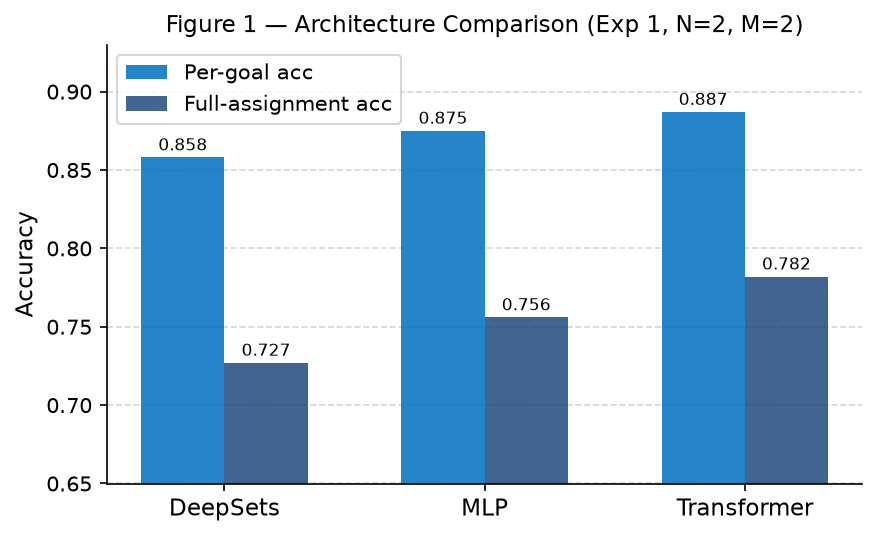
\includegraphics[width=0.82\textwidth]{fig1_arch.png}
\caption{Architecture comparison (Exp 1). The Transformer achieves the highest accuracy on both
metrics. The advantage over MLP widens from 1.7 pt at N=2 to 6.7 pt at N=5
(Table~\ref{tab:scale_n}).}
\label{fig:arch}
\end{figure}

\subsection{N-Scaling (Exp 2)}

\begin{table}[htbp]
\centering
\caption{Exp 2 --- full-assignment accuracy (per-goal in parentheses): N scaling, 8$\times$8, 10k train.}
\begin{tabularx}{\textwidth}{lXX}
\toprule
\textbf{N} & \textbf{MLP} & \textbf{Transformer} \\
\midrule
2 & $0.772 \pm 0.003$ (0.882) & $0.789 \pm 0.006$ (0.890) \\
3 & $0.549 \pm 0.005$ (0.812) & $0.590 \pm 0.004$ (0.830) \\
4 & $0.382 \pm 0.002$ (0.776) & $0.443 \pm 0.008$ (0.799) \\
5 & $0.270 \pm 0.002$ (0.758) & $0.337 \pm 0.004$ (0.785) \\
\bottomrule
\end{tabularx}
\label{tab:scale_n}
\end{table}

Full-assignment accuracy decays roughly as (per-goal)$^M$ for both models. The Transformer
gap over MLP grows monotonically with N, suggesting attention better handles the cross-goal
interdependencies that arise in larger problems.

\subsection{Capacity and Data-Scale (Exps 3--4)}

\begin{table}[htbp]
\centering
\caption{Exp 3 --- data-scale ablation: transformer h64/L3, N=3, 8$\times$8.}
\begin{tabularx}{\textwidth}{lXX}
\toprule
\textbf{Train size} & \textbf{Per-goal Acc} & \textbf{Full-assign Acc} \\
\midrule
1k  & $0.814 \pm 0.002$ & $0.553 \pm 0.003$ \\
5k  & $0.824 \pm 0.001$ & $0.578 \pm 0.001$ \\
10k & $0.831 \pm 0.003$ & $0.599 \pm 0.005$ \\
20k & $0.835 \pm 0.002$ & $0.603 \pm 0.003$ \\
\bottomrule
\end{tabularx}
\label{tab:datascale}
\end{table}

Gains flatten by 20k samples ($+$0.4 pt from 10k to 20k). Similarly, widening the hidden
dimension from 64 to 256 or deepening from L=3 to L=6 (Exp 4) adds at most $+$1.4 pt; h256/L6
diverges on some seeds at lr$=10^{-3}$. Together these results confirm that capacity and data
alone cannot close the accuracy gap --- the $G$ feature is the critical missing piece.

\subsection{Goal--Goal Distance Feature (Exp 5)}

\begin{table}[htbp]
\centering
\caption{Exp 5 --- $G$ ablation: transformer h64/L3, 8$\times$8, 10k train, 3 seeds.
Full-assignment accuracy.}
\rowcolors{2}{gray!8}{white}
\begin{tabularx}{\textwidth}{lXXX}
\toprule
\textbf{N} & \textbf{Without $G$} & \textbf{With $G$} & \textbf{Gain} \\
\midrule
2 & $0.790 \pm 0.002$ & $0.932 \pm 0.005$ & $+14.2$ pt \\
3 & $0.595 \pm 0.010$ & $0.775 \pm 0.008$ & $+18.0$ pt \\
4 & $0.455 \pm 0.006$ & $0.632 \pm 0.007$ & $+17.7$ pt \\
5 & $0.337 \pm 0.004$ & $0.478 \pm 0.011$ & $+14.1$ pt \\
\bottomrule
\end{tabularx}
\label{tab:ablation}
\end{table}

\begin{figure}[htbp]
\centering
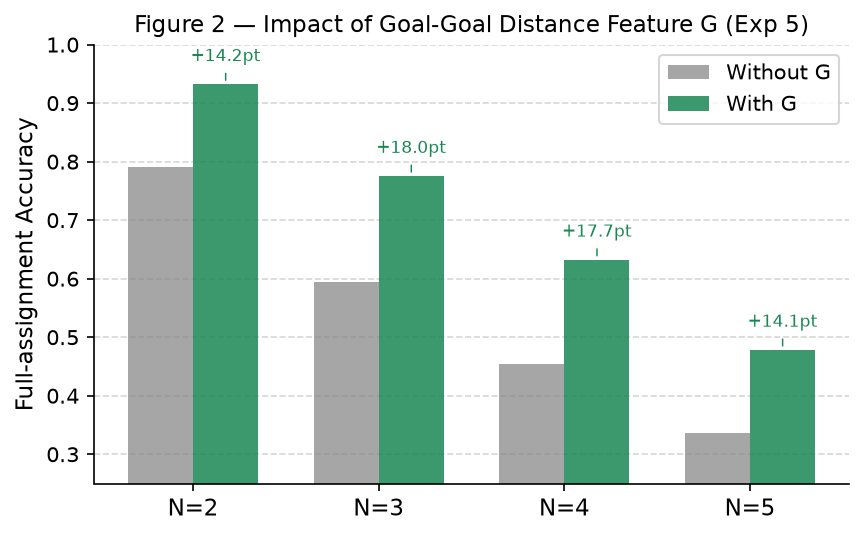
\includegraphics[width=0.82\textwidth]{fig2_ablation.png}
\caption{Adding goal-to-goal distances $G$ improves full-assignment accuracy by 14--18 pt at
every agent count. At N=2 with $G$, the mean cost ratio reaches 1.0000 --- near-perfect solver
agreement.}
\label{fig:ablation}
\end{figure}

\begin{findingbox}{Key Finding: Goal--Goal Distances Dominate}
The matrix $G$ provides the \emph{tour-structure signal} that $D$ alone cannot express: which
goals are adjacent and should be bundled to the same agent. A gain of $+14$--$18$ pt exceeds all
architecture, capacity, and data-scale improvements combined by $>10\times$. This was the
decisive design insight of the project.
\end{findingbox}

\subsection{Universal Mixed-Size Model (Exp 7)}

\begin{table}[htbp]
\centering
\caption{Universal model (151k params, N$\in$\{2,3,4\}$\times$M$\in$\{2..6\}) vs.\
per-size specialists. Full-assignment accuracy, 3 seeds. N=5 is zero-shot.}
\begin{tabularx}{\textwidth}{lXXX}
\toprule
\textbf{Config} & \textbf{Per-size Specialist} & \textbf{Universal Model} & \textbf{$\Delta$} \\
\midrule
N=M=2 & $0.932 \pm 0.005$ & $0.913 \pm 0.002$ & $-1.9$ pt \\
N=M=3 & $0.775 \pm 0.008$ & $0.810 \pm 0.002$ & $+3.5$ pt \\
N=M=4 & $0.632 \pm 0.007$ & $0.656 \pm 0.007$ & $+2.4$ pt \\
N=M=5 \emph{(zero-shot)} & $0.478 \pm 0.011$ & $0.513 \pm 0.003$ & $+3.5$ pt \\
\bottomrule
\end{tabularx}
\label{tab:universal}
\end{table}

The universal model outperforms per-size specialists on all configurations except the easiest
(N=M=2, $-1.9$ pt), and achieves $+3.5$ pt on N=5 --- a configuration it was \emph{never
trained on}. Cross-configuration sharing acts as regularization, preventing the model from
over-specializing to any single $(N,M)$ pair and enabling genuine transfer to unseen sizes.

\subsection{Full-Pipeline Evaluation (Exps 9--10)}

\begin{table}[htbp]
\centering
\caption{Exp 9 --- end-to-end MAPF execution cost: NN pipeline vs.\ solver, 200 instances/config,
single-instance timing. Execution cost = CBS collision-free path length (true MAPF objective).}
\rowcolors{2}{gray!8}{white}
\begin{tabularx}{\textwidth}{lXXXXXX}
\toprule
\textbf{Config} & \textbf{Cost Ratio} & \textbf{Exact Match} & \textbf{Diff (steps)} &
  \textbf{NN ms} & \textbf{Solver ms} & \textbf{Speedup} \\
\midrule
n2m2 & 1.010 & 96.5\% & 0.08 & 9.6  & 16.2 & 1.7$\times$ \\
n3m3 & 1.007 & 97.0\% & 0.07 & 8.0  & 21.7 & 2.7$\times$ \\
n4m4 & 1.029 & 88.0\% & 0.27 & 9.2  & 28.3 & 3.1$\times$ \\
n2m4 & 1.020 & 88.5\% & 0.26 & 6.8  & 15.1 & 2.2$\times$ \\
n4m6 & 1.050 & 72.5\% & 0.69 & 10.0 & 36.3 & 3.6$\times$ \\
n2m6 & 1.063 & 64.0\% & 1.09 & 9.2  & 22.5 & 2.4$\times$ \\
\bottomrule
\end{tabularx}
\label{tab:pipeline9}
\end{table}

Two structural insights emerge. First, exact-cost match (64--97\%) is far higher than
exact-assignment match because many differing allocations achieve the same CBS execution cost
--- they are cost-equivalent ties. Second, single-instance speedup (1.7--3.6$\times$) is far
below batched allocation-only speedup ($\sim$10$^3\times$ in Exp 8): CBS path planning
dominates both pipelines and only the LKH call is saved. Speedup trends upward with $M$ as
the solver's TSP component grows while the NN forward pass remains constant-time.

\subsection{Large Model on Diverse Distribution (Exp 11)}

\begin{table}[htbp]
\centering
\caption{Exp 11 offline per-goal accuracy on the diverse test set (h128/L6, 3 seeds,
std$\approx$0.000). Full-assignment accuracy in parentheses.}
\small\setlength{\tabcolsep}{5.5pt}
\begin{tabular}{lccccccc}
\toprule
\textbf{N$\backslash$M} & \textbf{2} & \textbf{3} & \textbf{4} & \textbf{5} & \textbf{6} & \textbf{7} & \textbf{8} \\
\midrule
2 & 0.960 (.94) & 0.949 (.90) & 0.928 (.84) & 0.911 (.76) & 0.892 (.69) & 0.876 (.63) & 0.852 (.55) \\
3 & 0.930 (.89) & 0.926 (.85) & 0.915 (.79) & 0.897 (.71) & 0.881 (.65) & 0.864 (.57) & 0.850 (.51) \\
4 & 0.923 (.87) & 0.919 (.82) & 0.899 (.73) & 0.886 (.67) & 0.875 (.60) & 0.854 (.51) & 0.841 (.47) \\
5 & 0.921 (.86) & 0.910 (.79) & 0.903 (.73) & 0.887 (.65) & 0.877 (.58) & 0.860 (.51) & 0.845 (.44) \\
\bottomrule
\end{tabular}
\label{tab:exp11_offline}
\end{table}

Accuracy degrades gracefully with $M$ and is essentially flat across $N$. The N=5 row, which
was zero-shot for the small model, is now fully in-distribution and matches N=2 at every $M$.

\begin{table}[htbp]
\centering
\caption{Exp 11 full-pipeline summary: large model vs.\ small universal model (Exp 10), mean
over 28 configs, 200 instances each.}
\begin{tabularx}{\textwidth}{lXXX}
\toprule
\textbf{Metric} & \textbf{Small (Exp 10, 8$\times$8)} & \textbf{Large (8$\times$8)} & \textbf{Large (diverse)} \\
\midrule
Mean cost ratio  & $\sim$1.040 & 1.029         & \textbf{1.020} \\
Exact-cost match & $\sim$80\%  & 82.9\%        & \textbf{85.0\%} \\
Infeasible alloc & $<$0.5\%   & \textbf{0\%}  & \textbf{0\%} \\
Fallbacks needed & $<$0.5\%   & \textbf{0\%}  & \textbf{0\%} \\
Mean speedup     & $\sim$2.8$\times$ & 2.4$\times$ & 2.1$\times$ \\
\bottomrule
\end{tabularx}
\label{tab:exp11_summary}
\end{table}

\begin{figure}[htbp]
\centering
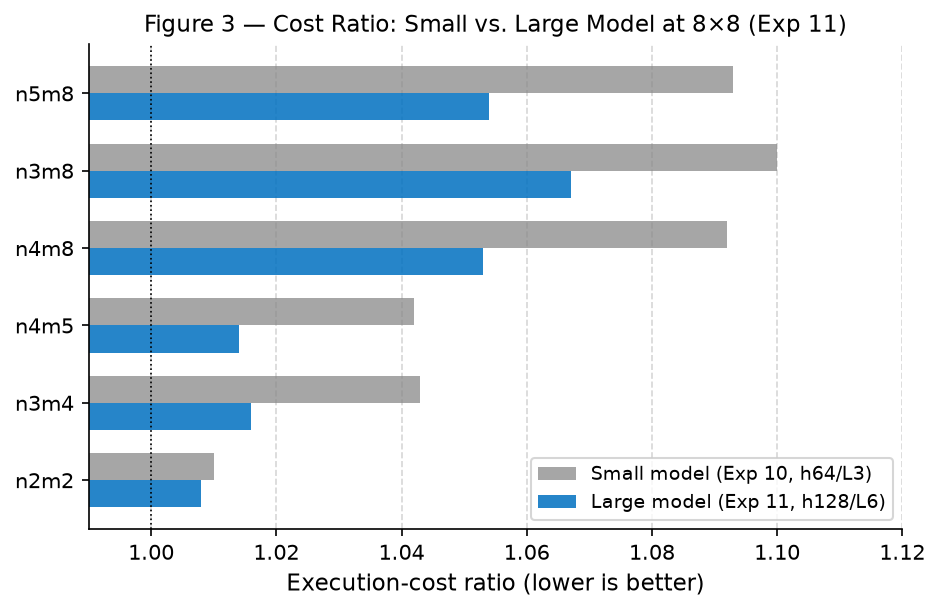
\includegraphics[width=0.85\textwidth]{fig3_exp11.png}
\caption{Cost ratio for selected configurations: small (Exp 10) vs.\ large (Exp 11) model.
Improvements concentrate on hard high-$M$ cells (e.g.\ n4m8: 1.092$\to$1.053;
n3m4: 1.043$\to$1.016). A dotted line marks ratio=1.0 (exact-solver agreement).}
\label{fig:exp11}
\end{figure}

The improvement of the large model concentrates on the hard, high-$M$ configurations where the
small model struggled most; easy small-$M$ configs move at most $\pm$1 pt. On its own
distribution the model achieves cost ratio 1.020, better than the off-distribution 8$\times$8
evaluation (1.029), confirming good generalization across grid geometries.

\subsection{Per-Configuration Breakdown: N$\times$M Heatmaps (Exp 11, diverse)}

Figures~\ref{fig:heatcost} and~\ref{fig:heatmatch} render the two headline metrics across the
full 28-configuration grid on the model's own diverse distribution. Both make the central
finding immediately visual: \textbf{the gradient runs horizontally, not vertically}. Difficulty
is driven almost entirely by the number of goals $M$ (each added goal is another per-goal
decision that must be correct), while the agent count $N$ leaves the metrics essentially flat ---
the same column colour holds from N=2 to N=5. The complete per-config tables backing these
heatmaps appear in Appendix~\ref{app:exp11}.

\begin{figure}[htbp]
\centering
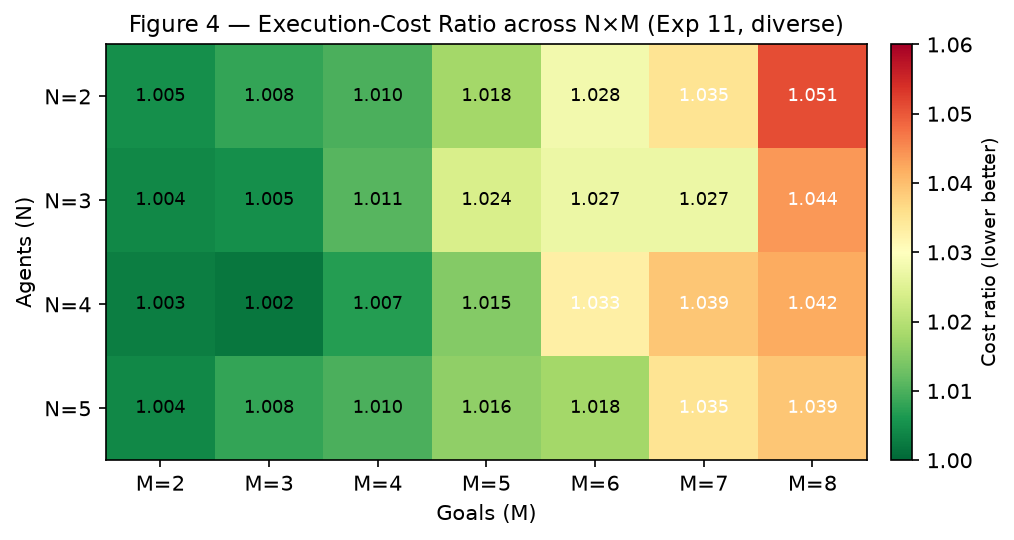
\includegraphics[width=0.88\textwidth]{fig4_heatmap_cost.png}
\caption{Execution-cost ratio across the N$\times$M grid (Exp 11, diverse distribution, 200
instances/config). Green = near-optimal (ratio $\to$1.0), red = costlier. The worst cell (n2m8,
1.051) is still within $\sim$5\% of the exact solver.}
\label{fig:heatcost}
\end{figure}

\begin{figure}[htbp]
\centering
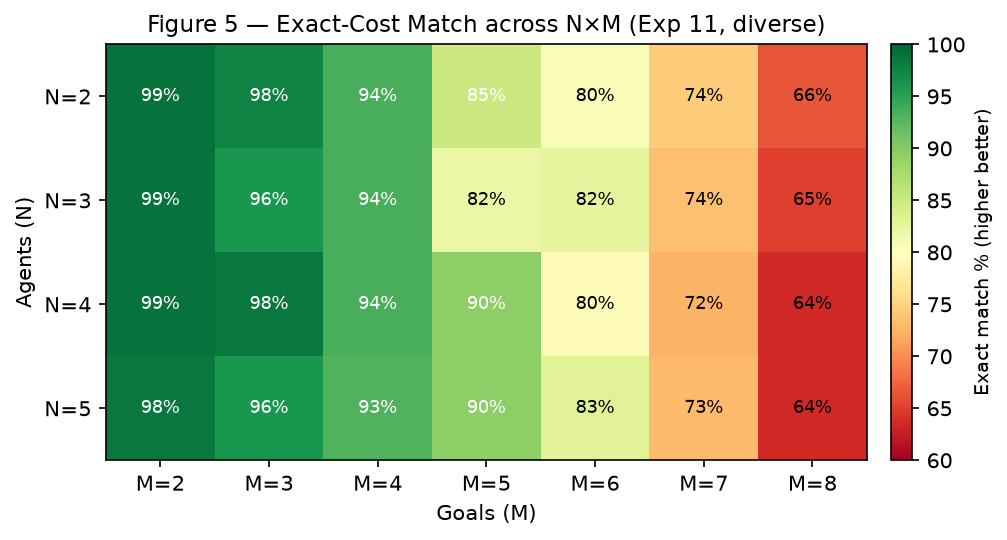
\includegraphics[width=0.88\textwidth]{fig5_heatmap_match.png}
\caption{Exact-cost-match fraction across the N$\times$M grid (Exp 11, diverse distribution).
Green = high agreement with the solver's execution cost. The 60--99\% range tracks $M$ almost
perfectly and is near-constant in $N$.}
\label{fig:heatmatch}
\end{figure}

\subsection{Training Convergence (Exp 11, large model)}

Figure~\ref{fig:convergence} traces the loss and per-goal accuracy of the h128/L6 model over its
150 training epochs, averaged across the three seeds (the $\pm1$ std bands are barely visible, so
the runs are highly reproducible). The two panels expose a clear \textbf{overfitting} regime that
shapes how the model is selected. Training loss falls monotonically from $0.39$ to $0.09$ and
training accuracy climbs to $0.969$, but the validation loss bottoms out at $\approx0.25$ around
epoch 22 and then \emph{rises} steadily to $\approx0.85$, while validation accuracy peaks near
$0.90$ and settles at $0.884$. The MinSum component stays essentially flat ($\approx0.257$)
throughout --- the movement is almost entirely in the cross-entropy term, i.e.\ the model is
progressively memorizing the solver's exact label on the training instances.

Because \texttt{train.py} checkpoints the weights at the \emph{minimum validation loss} rather
than the final epoch, the deployed model is effectively \textbf{early-stopped} at its epoch-22
optimum (best val loss $0.2514$/$0.2528$/$0.2537$ across seeds); all evaluation numbers in this
report come from that checkpoint, not the over-trained final state. The 150-epoch schedule is
therefore longer than strictly necessary --- accuracy and loss have both plateaued by epoch
$\sim$80 --- and a tighter early-stopping patience or stronger regularization is a natural lever
for future runs (see Next Steps).

\begin{figure}[htbp]
\centering
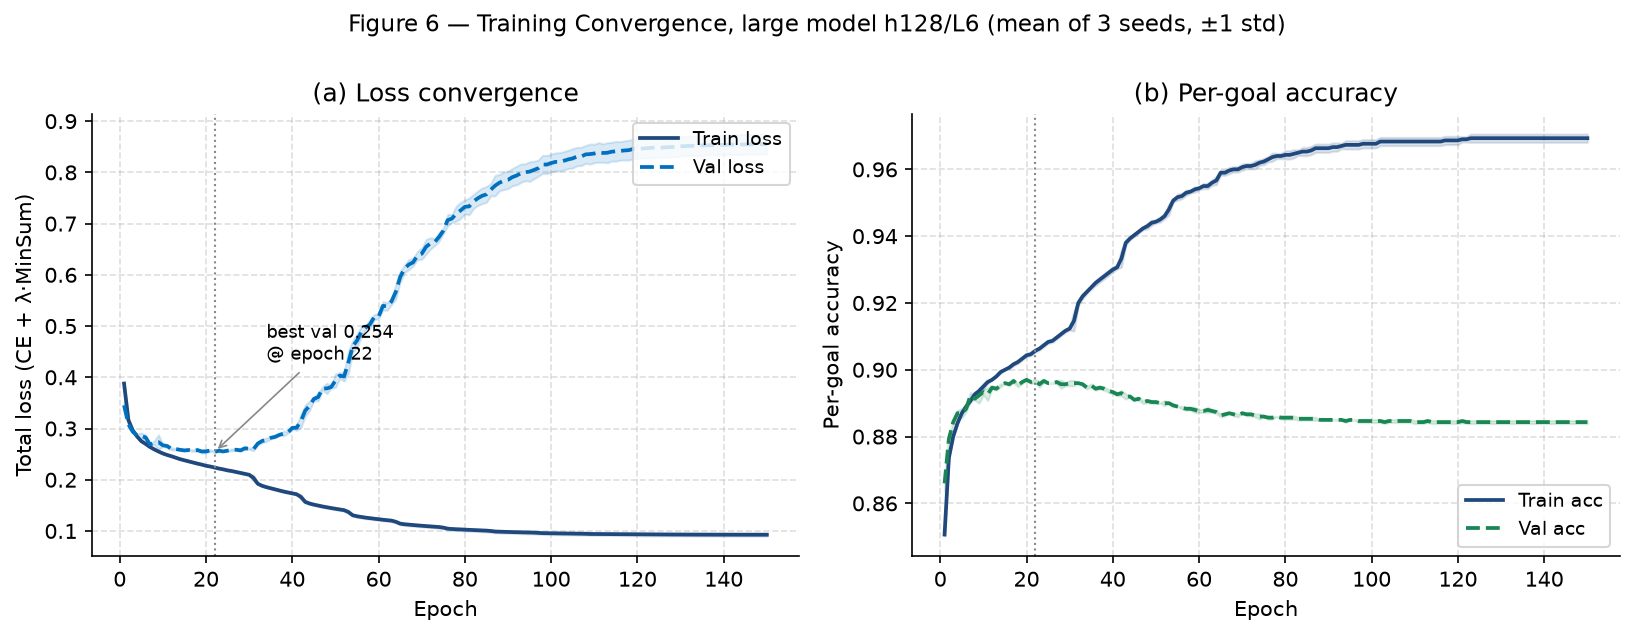
\includegraphics[width=\textwidth]{fig6_convergence.png}
\caption{Training convergence of the large model (h128/L6, mean of 3 seeds, $\pm1$ std).
\textbf{(a)} Total loss: train (solid) keeps falling while validation (dashed) turns upward after
its epoch-22 minimum --- the checkpoint is taken at that minimum (dotted line). \textbf{(b)}
Per-goal accuracy: the train/val gap widens after the same point. Both signatures are textbook
overfitting, controlled here by best-val-loss checkpointing.}
\label{fig:convergence}
\end{figure}

% ═════════════════════════════════════════════════════════════════════════════
\section{Full Per-Config Pipeline Tables (Exps 10--11)}
% ═════════════════════════════════════════════════════════════════════════════

The two full-pipeline sweeps are reproduced here in ascending experiment order: first the
Exp 10 baseline (small universal model, with zero-shot extrapolation cells), then the Exp 11
final model whose N$\times$M heatmaps appear in Figures~\ref{fig:heatcost}--\ref{fig:heatmatch}.

\subsection{Exp 10 --- small universal model (h64/L3), 8$\times$8}

\begin{longtable}{llccccc}
\caption{Complete Exp 10: universal model (h64/L3), 28 configs, 200 instances/config,
8$\times$8/10\% obstacles. ZS = zero-shot (N=5 or M$\geq$7).}
\label{tab:fullpipe10} \\
\toprule
\textbf{Config} & \textbf{ZS} & \textbf{Cost Ratio} & \textbf{Exact Match} &
  \textbf{Diff (steps)} & \textbf{NN ms} & \textbf{Speedup} \\
\midrule
\endfirsthead
\multicolumn{7}{c}{\small\textit{Table \ref{tab:fullpipe10} continued}} \\[4pt]
\toprule
\textbf{Config} & \textbf{ZS} & \textbf{Cost Ratio} & \textbf{Exact Match} &
  \textbf{Diff (steps)} & \textbf{NN ms} & \textbf{Speedup} \\
\midrule
\endhead
\bottomrule
\endfoot
n2m2 &              & 1.010 & 96.5\% & 0.07 & 11.3 & 3.0$\times$ \\
n2m3 &              & 1.006 & 98.0\% & 0.08 & 12.2 & 2.7$\times$ \\
n2m4 &              & 1.020 & 88.5\% & 0.26 & 12.7 & 2.5$\times$ \\
n2m5 &              & 1.044 & 74.5\% & 0.69 & 12.2 & 3.1$\times$ \\
n2m6 &              & 1.063 & 64.0\% & 1.09 & 17.0 & 2.3$\times$ \\
n2m7 & $\checkmark$ & 1.090 & 54.5\% & 1.61 & 18.3 & 2.1$\times$ \\
n2m8 & $\checkmark$ & 1.078 & 51.0\% & 1.55 & 38.7 & 1.1$\times$ \\
n3m2 &              & 1.009 & 98.0\% & 0.07 & 13.3 & 2.6$\times$ \\
n3m3 &              & 1.007 & 97.0\% & 0.07 & 12.1 & 2.6$\times$ \\
n3m4 &              & 1.043 & 83.0\% & 0.47 & 11.7 & 3.4$\times$ \\
n3m5 &              & 1.046 & 76.5\% & 0.60 & 12.3 & 3.2$\times$ \\
n3m6 &              & 1.070 & 66.5\% & 1.03 & 12.9 & 3.2$\times$ \\
n3m7 & $\checkmark$ & 1.068 & 58.0\% & 1.12 & 16.4 & 2.7$\times$ \\
n3m8 & $\checkmark$ & 1.100 & 43.5\% & 1.82 & 20.4 & 2.5$\times$ \\
n4m2 &              & 1.000 & 100.0\% & 0.00 & 10.9 & 3.1$\times$ \\
n4m3 &              & 1.010 & 96.0\% & 0.09 & 11.7 & 3.2$\times$ \\
n4m4 &              & 1.029 & 88.0\% & 0.27 & 12.1 & 3.3$\times$ \\
n4m5 &              & 1.042 & 76.0\% & 0.54 & 12.8 & 3.5$\times$ \\
n4m6 &              & 1.050 & 72.5\% & 0.69 & 13.3 & 3.5$\times$ \\
n4m7 & $\checkmark$ & 1.074 & 55.5\% & 1.09 & 19.8 & 2.5$\times$ \\
n4m8 & $\checkmark$ & 1.092 & 40.0\% & 1.52 & 19.6 & 2.7$\times$ \\
n5m2 & $\checkmark$ & 1.002 & 99.5\% & 0.01 & 34.8 & 1.1$\times$ \\
n5m3 & $\checkmark$ & 1.009 & 96.5\% & 0.07 & 30.1 & 1.3$\times$ \\
n5m4 & $\checkmark$ & 1.020 & 91.5\% & 0.19 & 13.3 & 3.3$\times$ \\
n5m5 & $\checkmark$ & 1.041 & 76.5\% & 0.47 & 41.5 & 1.2$\times$ \\
n5m6 & $\checkmark$ & 1.053 & 73.0\% & 0.67 & 14.3 & 3.9$\times$ \\
n5m7 & $\checkmark$ & 1.070 & 52.5\% & 0.98 & 15.5 & 4.1$\times$ \\
n5m8 & $\checkmark$ & 1.093 & 38.5\% & 1.49 & 17.4 & 3.8$\times$ \\
\end{longtable}

\subsection{Exp 11 --- large model (h128/L6), diverse distribution}
\label{app:exp11}

\begin{longtable}{lcccc}
\caption{Complete Exp 11: large model (h128/L6), 28 configs, 200 instances/config, on its own
diverse distribution (grids 8--12, walls 0.1--0.5). All configs in-distribution (no
extrapolation column). These are the values plotted in
Figures~\ref{fig:heatcost}--\ref{fig:heatmatch}.}
\label{tab:fullpipe11} \\
\toprule
\textbf{Config} & \textbf{Cost Ratio} & \textbf{Exact Match} & \textbf{Diff (steps)} & \textbf{Speedup} \\
\midrule
\endfirsthead
\multicolumn{5}{c}{\small\textit{Table \ref{tab:fullpipe11} continued}} \\[4pt]
\toprule
\textbf{Config} & \textbf{Cost Ratio} & \textbf{Exact Match} & \textbf{Diff (steps)} & \textbf{Speedup} \\
\midrule
\endhead
\bottomrule
\endfoot
n2m2 & 1.005 & 99.0\% & 0.04 & 1.9$\times$ \\
n2m3 & 1.008 & 97.5\% & 0.12 & 1.9$\times$ \\
n2m4 & 1.010 & 93.5\% & 0.17 & 1.7$\times$ \\
n2m5 & 1.018 & 85.0\% & 0.42 & 1.8$\times$ \\
n2m6 & 1.028 & 80.5\% & 0.66 & 2.1$\times$ \\
n2m7 & 1.035 & 74.5\% & 0.81 & 2.1$\times$ \\
n2m8 & 1.051 & 66.5\% & 1.39 & 1.3$\times$ \\
n3m2 & 1.004 & 99.0\% & 0.04 & 2.2$\times$ \\
n3m3 & 1.005 & 96.0\% & 0.06 & 1.9$\times$ \\
n3m4 & 1.011 & 93.5\% & 0.17 & 2.1$\times$ \\
n3m5 & 1.024 & 82.0\% & 0.49 & 2.0$\times$ \\
n3m6 & 1.027 & 82.5\% & 0.55 & 2.3$\times$ \\
n3m7 & 1.027 & 73.5\% & 0.55 & 2.1$\times$ \\
n3m8 & 1.044 & 65.0\% & 1.08 & 2.1$\times$ \\
n4m2 & 1.003 & 99.0\% & 0.02 & 2.6$\times$ \\
n4m3 & 1.002 & 98.5\% & 0.02 & 2.2$\times$ \\
n4m4 & 1.007 & 93.5\% & 0.09 & 2.3$\times$ \\
n4m5 & 1.015 & 89.5\% & 0.25 & 0.6$\times$ \\
n4m6 & 1.033 & 79.5\% & 0.63 & 2.3$\times$ \\
n4m7 & 1.039 & 72.5\% & 0.81 & 2.4$\times$ \\
n4m8 & 1.042 & 63.5\% & 0.97 & 2.7$\times$ \\
n5m2 & 1.004 & 98.5\% & 0.02 & 2.3$\times$ \\
n5m3 & 1.008 & 96.0\% & 0.08 & 2.4$\times$ \\
n5m4 & 1.010 & 93.0\% & 0.15 & 2.5$\times$ \\
n5m5 & 1.016 & 89.5\% & 0.22 & 1.1$\times$ \\
n5m6 & 1.018 & 83.0\% & 0.34 & 2.3$\times$ \\
n5m7 & 1.035 & 73.0\% & 0.67 & 2.8$\times$ \\
n5m8 & 1.039 & 63.5\% & 0.83 & 2.7$\times$ \\
\end{longtable}

\clearpage
% ═════════════════════════════════════════════════════════════════════════════
\section{Real Benchmark Maps and Training-Data Study (Exps 12--15)}
% ═════════════════════════════════════════════════════════════════════════════

The second phase replaces procedural grids with the four 32$\times$32 RobustMCPF benchmark maps and
scales to N$\in$\{5,10,15\}, M$\in$\{10,20,30\}. Figure~\ref{fig:maps} shows the four maps, spanning
open geometry to highly structured corridors.

\begin{figure}[H]
\centering
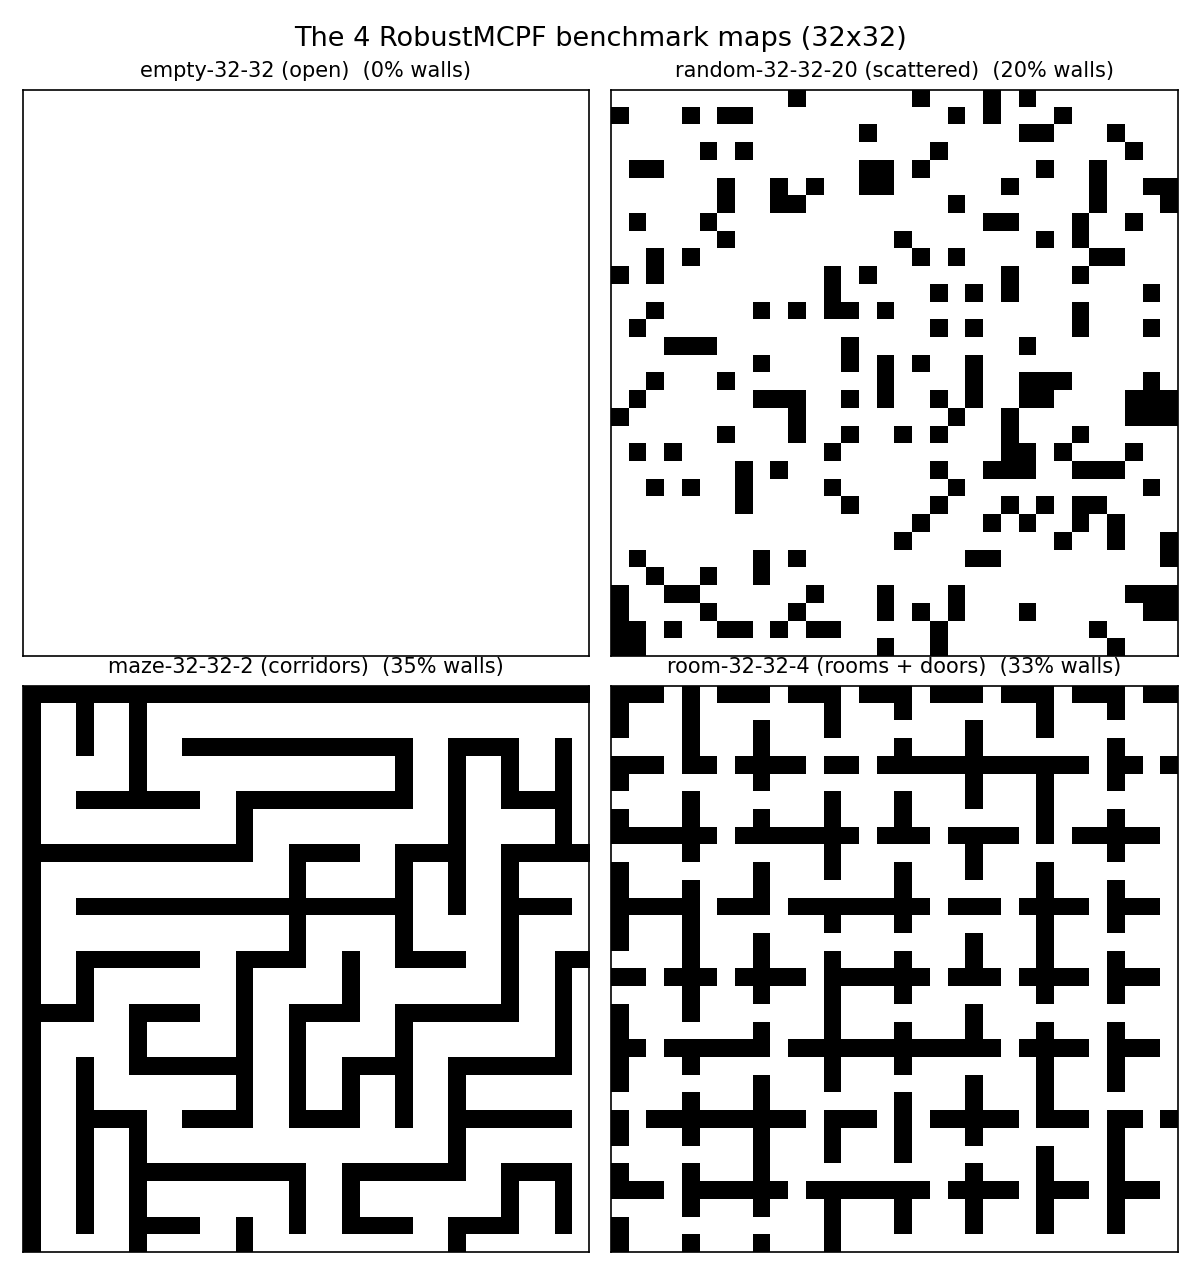
\includegraphics[width=0.74\textwidth]{maps/maps_panel.png}
\caption{The four 32$\times$32 benchmark maps. Only \texttt{maze} and \texttt{room} carry
\emph{structured} (corridor/room) geometry --- the distinction that drives the Exp 14 result.}
\label{fig:maps}
\end{figure}

\subsection{Map-Trained Models: h128 vs h256 (Exp 12)}
Two universal models (the Exp-11 architecture) were trained directly on the four maps at the new
scale. In-distribution the smaller \textbf{h128} model wins (mean execution-cost ratio
\textbf{1.048} vs 1.052 for h256) --- the extra capacity overfits rather than helping. As
throughout, difficulty tracks $M$, not $N$.

\subsection{Does the Old Model Transfer? (Exps 13.a, 13.b)}
Exp~13.a evaluates the Exp-11 model (\emph{trained only on small random grids}) zero-shot on the
real maps at small N/M: it transfers cleanly --- mean ratio \textbf{1.019}, and structured maps are
\emph{easier} than open ones because walls remove allocation ties. Exp~13.b pushes the same model to
the large-N/M regime, where it \emph{fails to extrapolate}: mean ratio \textbf{1.246} versus the
map-trained B1's 1.048. The signature is a scissors (Figure~\ref{fig:scissors}): at M=30, adding
agents \emph{hurts} the old model (trained on N$\le$5) but \emph{helps} the in-range B1.

\begin{figure}[H]
\centering
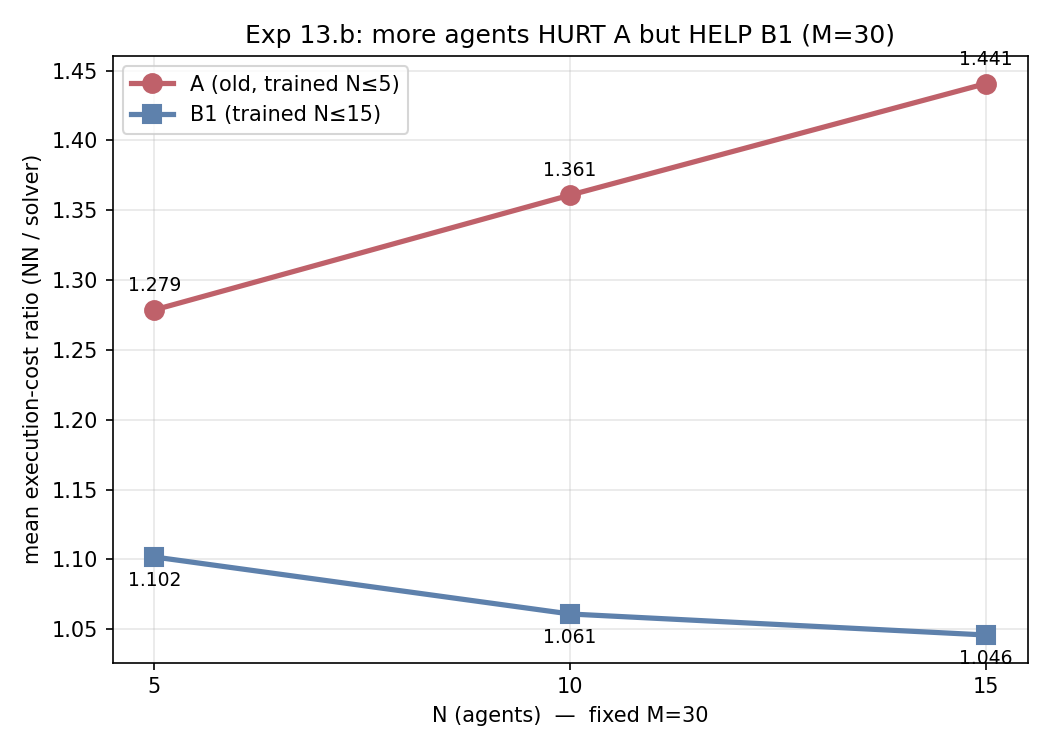
\includegraphics[width=0.6\textwidth]{oldmodel_large_nm/fig2_N_divergence_m30.png}
\caption{Exp 13.b: at M=30, more agents hurt the old model A (trained N$\le$5) but help the
map-trained B1 (trained N$\le$15). Generalization fails across \emph{scale}, not geometry.}
\label{fig:scissors}
\end{figure}

\subsection{Random-Diverse vs Fixed-Map Training (Exp 14)}
A controlled study: models \textbf{C} copy the \textbf{B} recipe exactly, swapping only the training
data --- random 32$\times$32 grids with 0--50\% wall density instead of the four fixed maps.
Fixed-map training wins overall (h128 1.048 vs 1.075), but \textbf{the entire gap is the maze}
(Figure~\ref{fig:cvsb}); on open/scattered/room maps the two tie. Random Bernoulli walls resemble
those maps but never reproduce the maze's corridor structure.

\begin{figure}[H]
\centering
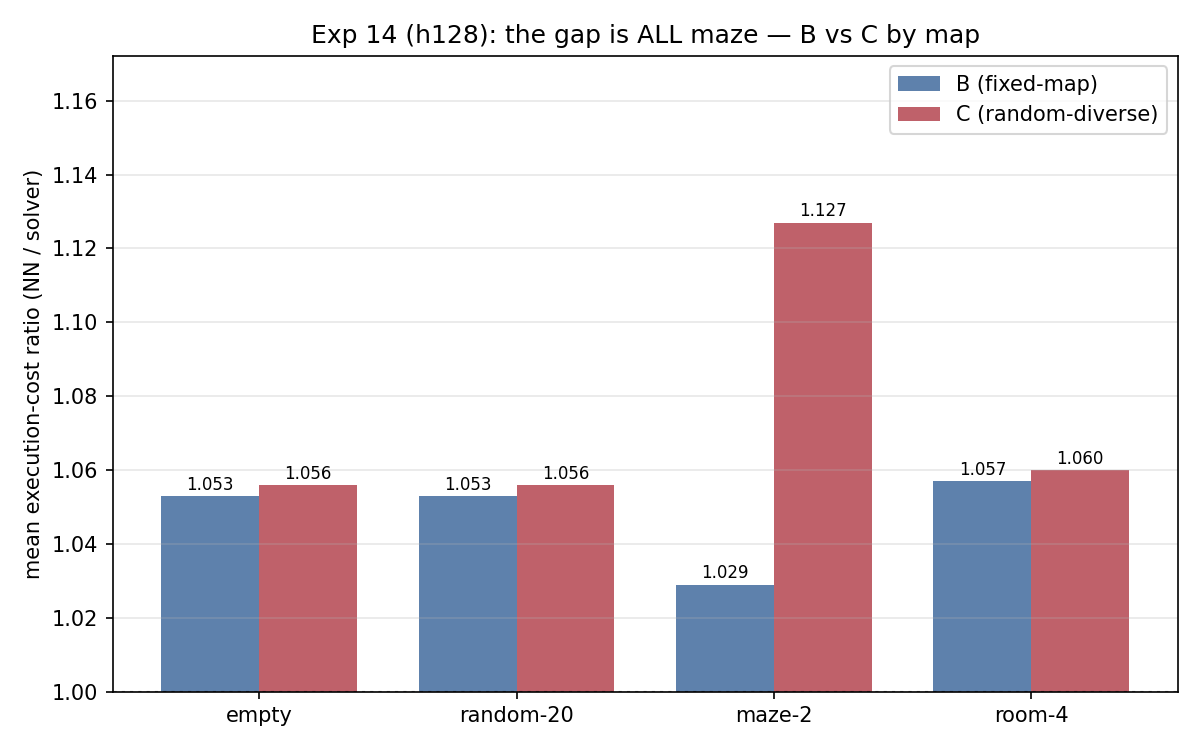
\includegraphics[width=0.78\textwidth]{random_vs_fixed/fig1_by_map_h128.png}
\caption{Exp 14 (h128): random-diverse training (C) ties fixed-map training (B) on every map
\emph{except} the maze, where it never saw corridor structure.}
\label{fig:cvsb}
\end{figure}

\subsection{Zero-Shot XL Extrapolation (Exp 15)}
The Exp-14 winner (the fixed-map family) is pushed far beyond its training range to paper scale,
N$\in$\{20,35,50\}$\times$M$\in$\{50,75,100\} (toward the paper's N$\le$50/M$\le$100), with no
retraining. Here the in-distribution verdict \emph{flips}: the larger \textbf{h256} model
extrapolates better (mean cost ratio \textbf{1.208} vs 1.244 for h128) and roughly halves the
worst-case gap, while single-instance speedup climbs to \textbf{5.9--9.4$\times$} as the solver's
TSP/CBS workload grows. The capacity that merely overfit in range becomes the better generalizer at
scale --- and this is the regime where replacing the exact solver yields the largest speed win.

\begin{findingbox}{Phase-Two Conclusion}
Training data matters for \emph{structured} geometry only. The old model generalizes across map
shape but not problem scale; random-grid training is a free substitute for fixed-map training on
unstructured maps but loses on the maze. At extreme scale (Exp 15) the larger model extrapolates
best and runs \textbf{5.9--9.4$\times$} faster than the solver --- the operating point where replacing
the exact solver is most worthwhile.
\end{findingbox}

% ═════════════════════════════════════════════════════════════════════════════
\section{Summary: The Model and Where It Helps}
% ═════════════════════════════════════════════════════════════════════════════

\textbf{How it works.} Each instance is encoded as numeric matrices --- the agent$\to$goal BFS
distances $D\in\mathbb{R}^{N\times M}$ and goal$\to$goal distances $G\in\mathbb{R}^{M\times M}$. The
universal transformer processes them with alternating row/column attention (no positional
embeddings, so it accepts \emph{any} $N,M$) and emits a column-wise softmax
$P\in\mathbb{R}^{N\times M}$ --- for each goal, a distribution over agents. An arg-max decode yields
the allocation, which a classical goal-ordering and CBS step turns into collision-free paths. In
short: \emph{problem $\to$ ($D,G$) vectors $\to$ attention $\to$ per-goal probabilities $\to$
allocation $\to$ paths}.

\textbf{Small vs.\ large model.} Two sizes were studied: \textbf{h128/L6} (1.2M params) and
\textbf{h256/L8} (6.3M). In-distribution the small model is both more accurate and faster --- the
large one overfits (Exp 12). Far out-of-distribution the ranking reverses: the large model is the
better extrapolator (Exp 15). Practically, prefer h128 when deployment matches the training range
and h256 when heavy extrapolation beyond it is expected.

\textbf{When to use the NN instead of the exact solver.} The network replaces only the
combinatorial \emph{allocation} step (LKH-TSP); collision planning (CBS) is shared by both
pipelines. Its advantage therefore appears where allocation/TSP cost dominates and where many
instances must be solved: (i) \emph{large $N,M$}, where LKH grows expensive and the NN gives
\textbf{5.9--9.4$\times$} speedup at $\sim$20\% cost overhead (Exp 15); (ii) \emph{batched,
high-throughput} use, where allocation-only inference is orders of magnitude faster; and
(iii) \emph{unstructured geometry}, where even cheap random-grid training transfers (Exp 14).
Conversely, on small instances the exact solver is already millisecond-fast with few collisions, so
the NN offers no speed benefit (Exp 13.a); and on \emph{structured} maps it must be trained on that
geometry to stay competitive (the maze lesson, Exp 14). The NN is thus best understood as a fast,
\emph{near-optimal} drop-in for the allocation oracle ($\sim$1--6\% over optimal in range,
$\sim$20\% at extreme scale) for use when speed and scale matter more than exactness.

% ═════════════════════════════════════════════════════════════════════════════
\section{Next Steps}
% ═════════════════════════════════════════════════════════════════════════════

\textbf{Tour-aware loss.} The solver's true mTSP cost is computed during data generation and
currently discarded. Storing it per sample is a one-line change to \texttt{build\_dataset.py}.
A tour-chain regularizer $\sum_{j,k}(\sum_i P_{ij}P_{ik})G_{jk}$ would directly penalize
splitting adjacent goals across agents, targeting the M-difficulty axis.

\textbf{Learned goal-visit ordering.} Replacing the $k!$ brute-force enumeration with a learned
ordering head would eliminate the latency spike at high $k$ and extend the NN's speed advantage
to arbitrary $M$ without the $k=7/8$ outlier problem.

\textbf{Curb the overfitting.} The convergence curves (Figure~\ref{fig:convergence}) show
validation loss diverging after epoch $\sim$22 while training loss keeps falling. Best-val-loss
checkpointing already captures the right model, but explicit early stopping (e.g.\ patience
$\sim$20), weight decay, or dropout would shorten the 150-epoch schedule and likely lift the
validation plateau itself rather than just stopping at it.

\textbf{Collision-aware training.} CBS execution cost is not differentiable, but approximate
conflict penalties or policy-gradient signals could move training toward optimizing the true
MAPF objective rather than the allocation-imitation proxy.

\textbf{Report figures from raw data.} The per-instance CSVs from Exp 11 on the cluster (5,600
rows total: \texttt{results/fullpipe\_large/} and \texttt{results/fullpipe\_large\_diverse/})
support standard-deviation and percentile analyses without re-running any experiments.
Generating final report-quality figures from this raw data is the immediate documentation task.

\end{document}
